%%%%%%%%%%%%%%%%%%%%%%%%%%%%%%%%%%%%%%%%%%%%%%%%%
%%%%%%%%%%%% cap: theory %%%%%%%%%%%%%%%%%
%%%%%%%%%%%%%%%%%%%%%%%%%%%%%%%%%%%%%%%%%%%%%%%%%

\chapter{Theoretical Basis}\label{cap:theory}
To fully understand this paper and the development of its proposed solution, it is necessary to first understand some basic concepts and the theory regarding the current context. The purpose of this second chapter is to describe and explain notions regarding the subject at hand and to give examples of how they fit into the proposed solution.


%%%%%%%%%%%%%%%%%%%%%%%%%%%%%%%%%%%%%%%%%%%%%
%%%%%%%%%%%% Section: Neurotechs %%%%%%%%%%%%
%%%%%%%%%%%%%%%%%%%%%%%%%%%%%%%%%%%%%%%%%%%%%
\section{Neurotechnology}
\subsection{Electroencephalography (EEG)}
Electroencephalography or EEG is a method of recording an electrogram of the brain's spontaneous electrical activity. Brain cells communicate via electrical impulses and are active all the time, even during sleep\cite{EEG_mayoclinic}. This activity shows up as wavy lines on an EEG recording[see Fig 2.1]. For the purpose of realising this thesis I am using a non-invasive EEG method via the electrodes provided with the Unicorn Hybrid Black BCI[see fig 2.2].

\begin{figure}[H]
    \begin{minipage}[c]{0.45\linewidth}
      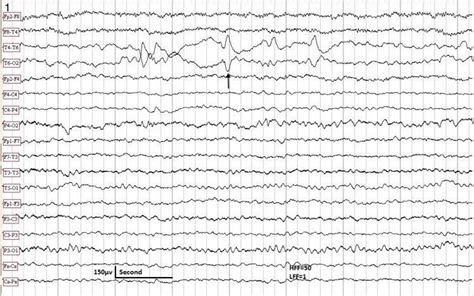
\includegraphics[width=\linewidth]{Graphics/EEG Example.jpeg}
      \caption{Sample EEG}
      \end{minipage}
    \hfill
    \begin{minipage}[c]{0.45\linewidth}
      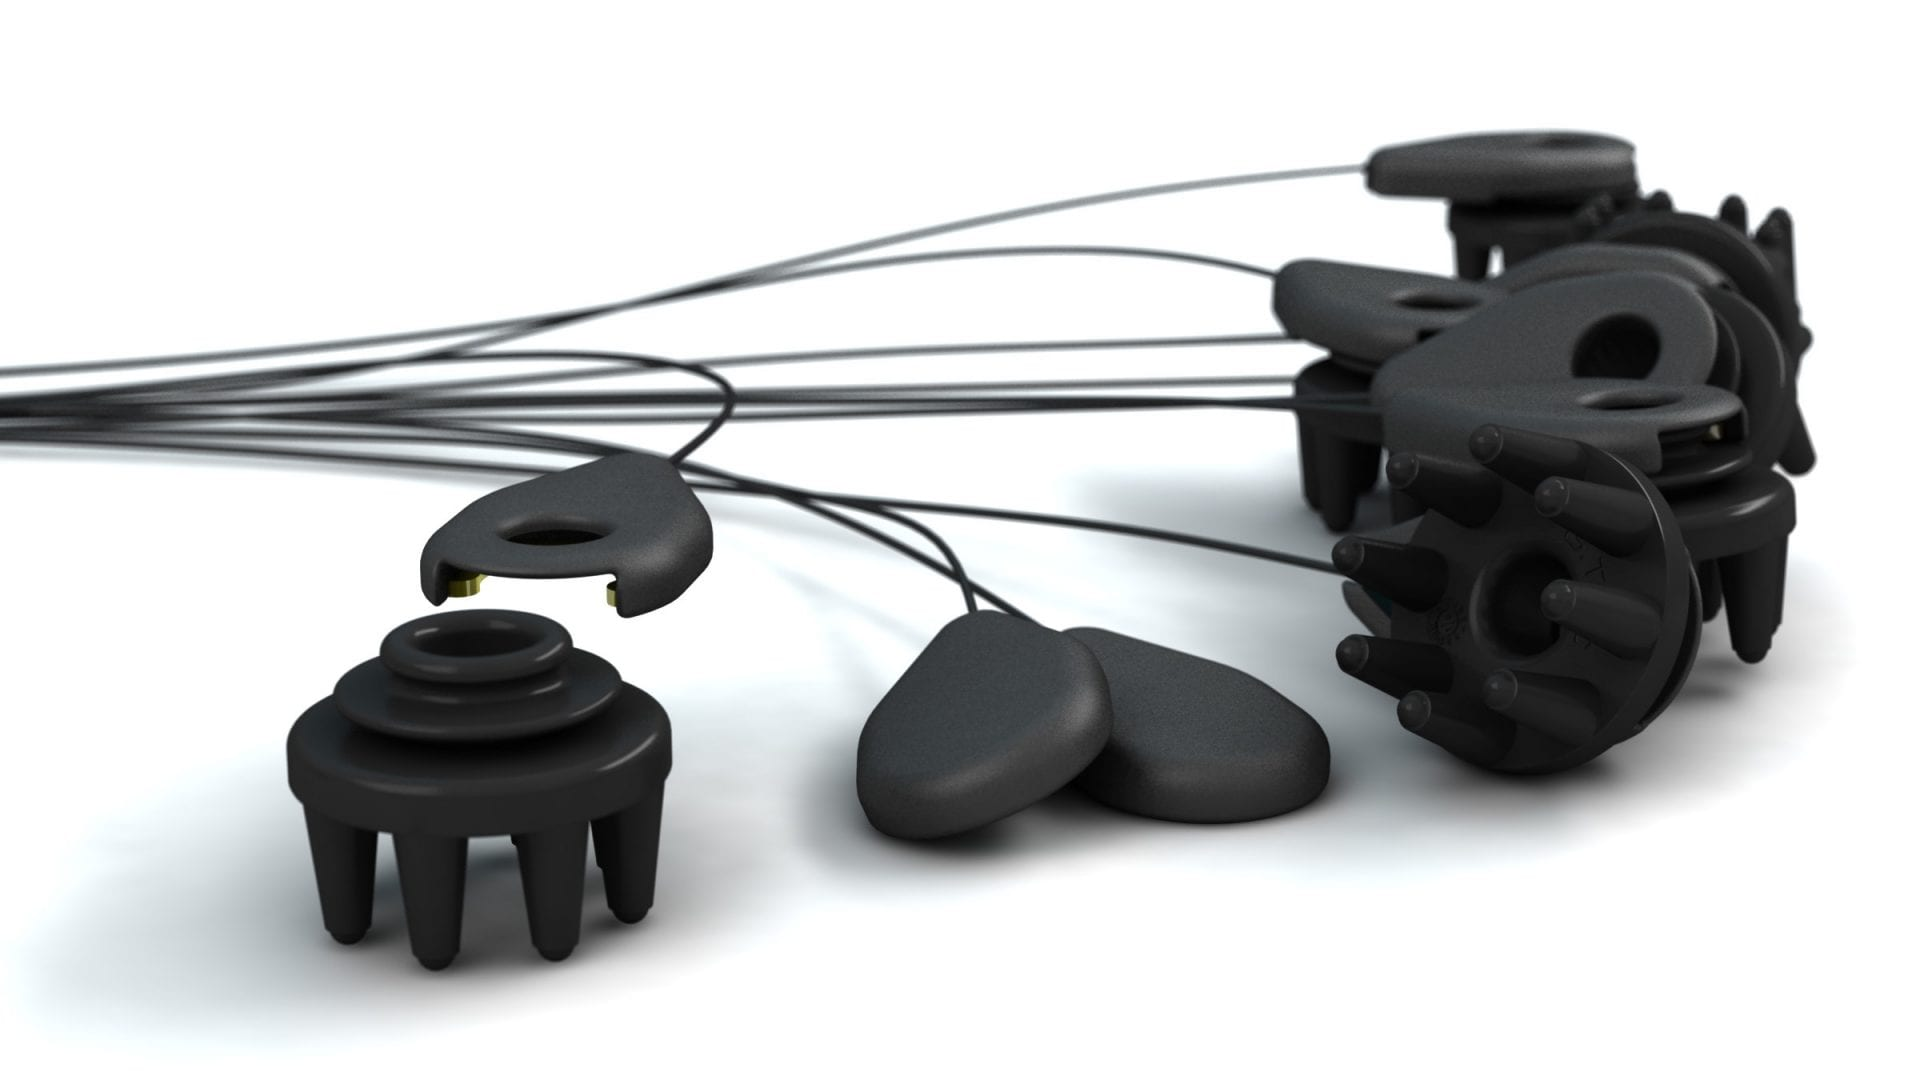
\includegraphics[width=\linewidth]{Graphics/Unicorn Electrodes.jpg}
      \caption{Unicorn Electrodes}
  \end{minipage}%
\end{figure}

Non-invasive EEG methods measure voltage fluctuations at the scalp which are produced by neuronal activity in the brain, but it is difficult to trace these signals back to the brain. As such, EEGs have low special resolution and are unable to provide precise information. Coupled with signal noise from various sources (electrical interference, muscle activity, eye movements, etc.) and interference from the skin and the skull, this makes the EEG a very sensitive tool. This can make results vary greatly, with the same user sometimes generating different results in the same testing medium. The signals may also get weaker and less accurate over time due to the user's state of mind and body (level of alertness, mental fatigue, physical fatigue, etc.) and the user may move the electrodes involuntarily as they are in use through normal body movement. There is also a case to be made about the comfort of the user which can play a vital role in getting the best results, as an uncomfortable user will pay less attention to the task at hand and thus generate more noise, inaccuracies and instability in an already sensitive system.


\subsection{P300}
The P300 is a component of event-related potential (ERP) used in decision-making. It is used in measuring the user's reaction to an external stimulus. It is implemented using the Oddball Paradigm, an experimental design in psychological research, where the stimulus to be observed is introduced between other redundant stimuli.

\subsection{Brain-Computer Interfacing}
A brain-computer interface(BCI) or brain-machine interface(BMI) is a computer-based system that acquires brain signals, analyses them and translates them into usable data or commands which are then exported to other devices to be used to other extents. By definition, a BCI uses some form or another of data processing and as such an EEG alone cannot be called a BCI\cite{Shih_2012}. BCI implementations vary based on the invasiveness of their data acquisition methods. As such, there are non-invasive BCIs (using electroencephalography, magnetoencephalography, electrooculography or magnetic resonance imaging), semi-invasive BCIs (using electrocorticography and endovascular methods) and invasive BCIs (using microelectrode arrays).

\subsection{Unicorn Hybrid Black BCI}
The BCI that will be used in the implementation of this paper is the Unicorn Hybrid Black. This is a non-invasive BCI using EEG technology. The 8 electroencephalogram electrodes are placed at the following fixed positions on the provided cap: Fz, C3, Cz, C4, Pz, PO7, Oz and PO8[see fig 2.3], in accordance with the 10/20 international system. Two extra electrodes marked L and R are to be attached to the mastoid bones behind the user's ears and act as a "ground" for the rest of the electrodes due to their placement on an area with virtually no electrical activity. 

\begin{figure}[H]
  \centering
  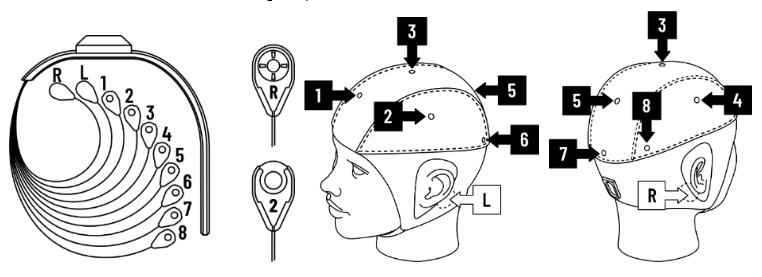
\includegraphics[width=0.8\textwidth]{Graphics/Electrode Placement.png}
  \caption{Electrode placement on the cap}
\end{figure}

The EEG cap works with 8 channels(with 2 extra "ground" channels) on a 24-bit resolution and a refresh rate of 250 hertz. The data is outputted via Bluetooth to a computer where it is processed.


%%%%%%%%%%%%%%%%%%%%%%%%%%%%%%%%%%%%%%%%%%%%%
%%%%%%%%%%%% Section: Techs %%%%%%%%%%%%%%%%%
%%%%%%%%%%%%%%%%%%%%%%%%%%%%%%%%%%%%%%%%%%%%%
\section{Technologies Used}
\subsection{Unicorn Suite}
The Unicorn BCI always comes alongside the Unicorn Suite, a software environment touched upon in the similar solutions section of this paper. In this implementation, the suite is used for its development tools and the Unicorn Speller contained within. Other useful tools include the Unicorn recorder, the .NET framework which uses the C\# programming language and other tools that allow the creation of different software solutions. Another function of the Suite is to keep the licenses required to use the software, as most tools require licenses purchased directly from g.tec\cite{Unicorn_Shop}, including the Speller used in this implementation.


\subsection{Unicorn Speller}
The Unicorn Speller is a spelling system that uses the P300 complex\cite{UnicornSuite_Manual}. The speller's interface consists of a QWERTY key layout that sits on the screen along a number row, an auto-complete row and a special functions row[see Fig 2.4]. The numbers and letters are used for spelling while the special keys are used for other functions such as text-to-speech, printing, etc. Each key is considered an item, and the layout is called a board. The user can choose the board he/she wants to use, thus choosing the layout of the items on the screen. The speller also allows for the creation of user-made boards (using the \textit{.ibc} file extension), the use of which will also be employed in this work. 
\vspace{\baselineskip}\newline
The actual mode of operation of the speller is through "flashing"\cite{UnicornSuite_Manual}, where the items on the board are flashing a different image for a brief moment (eg. the letter S is replaced with the face of Chuck Norris for a brief second before returning to its normal appearance). The images that flash on the letters are usually the faces of famous people. This is due to discoveries regarding P300 spellers, where researchers found out that superimposing familiar faces on letters helps accuracy and improves the performance of the ERP\cite{Li_2015}\cite{Kaufmann_2011}. To select an item, the user must focus on said item and count each time the item he/she wants to select flashes and ignore all other flashes\cite{UnicornSuite_Manual}.

\begin{figure}[H]
  \centering
  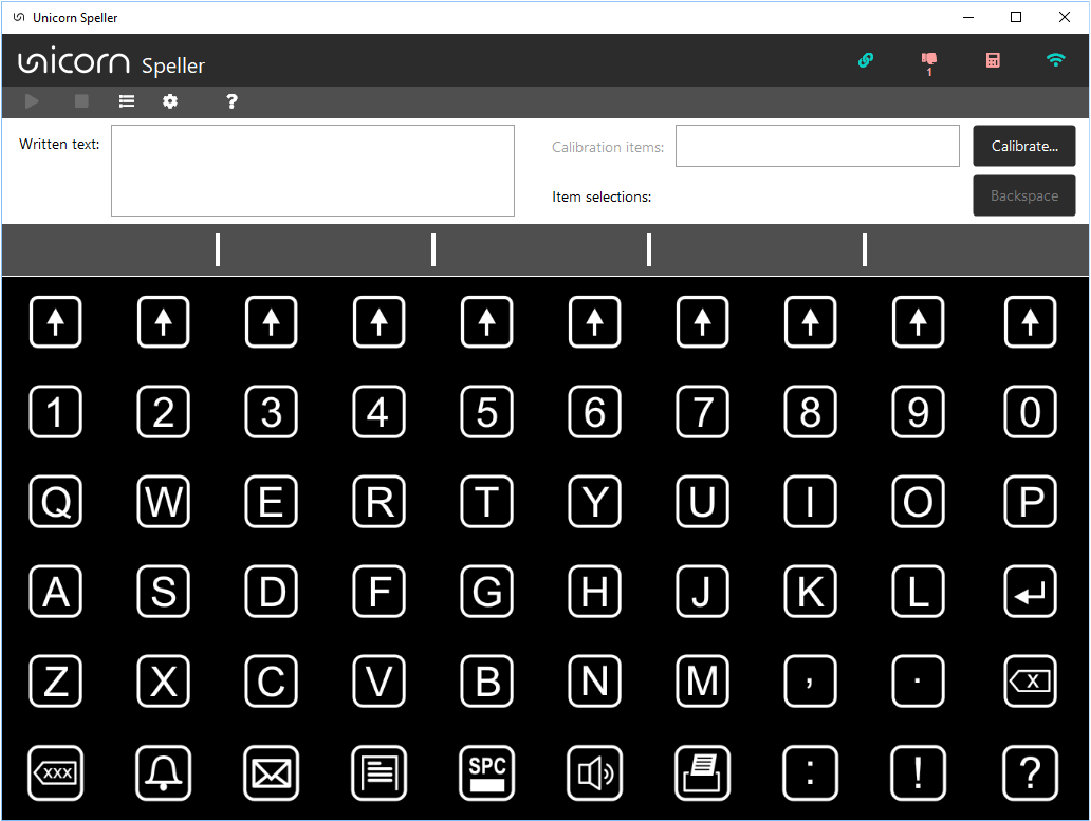
\includegraphics[width=1\textwidth]{Graphics/Speller.png}
  \caption{Unicorn speller using the default board}
\end{figure}

The speller flashing occurs in flash cycles, a group of flashes such as that each item on the board has flashed exactly once. There are different modes of flashing that the user can choose from as follows: row/column, single character and randomised patterns. To create the solution proposed by this paper, I will be using the randomised patterns mode, a randomised selection of items distributed across the whole board that flash at the same time, with patterns flashing consecutively\cite{UnicornSuite_Manual}. 
\vspace{\baselineskip}\newline
Furthermore, to use the speller, a calibration sequence needs to be completed. To calibrate, we must input a word or different letters that the user has to look at while the calibration sequence runs[see Fig 2.4]. During calibration, the speller learns the difference between the user's typical EEG signals and afterwards, it creates a calibration file, storing the user's calibration data to be reused. In this way, the speller adapts to the user, each user having different calibrations depending on different variables such as the user's environment. Therefore, it is best to calibrate in a quiet place, away from distractions and disturbances that might introduce rubbish data and noise in the calibration file.

\begin{figure}[H]
  \centering
  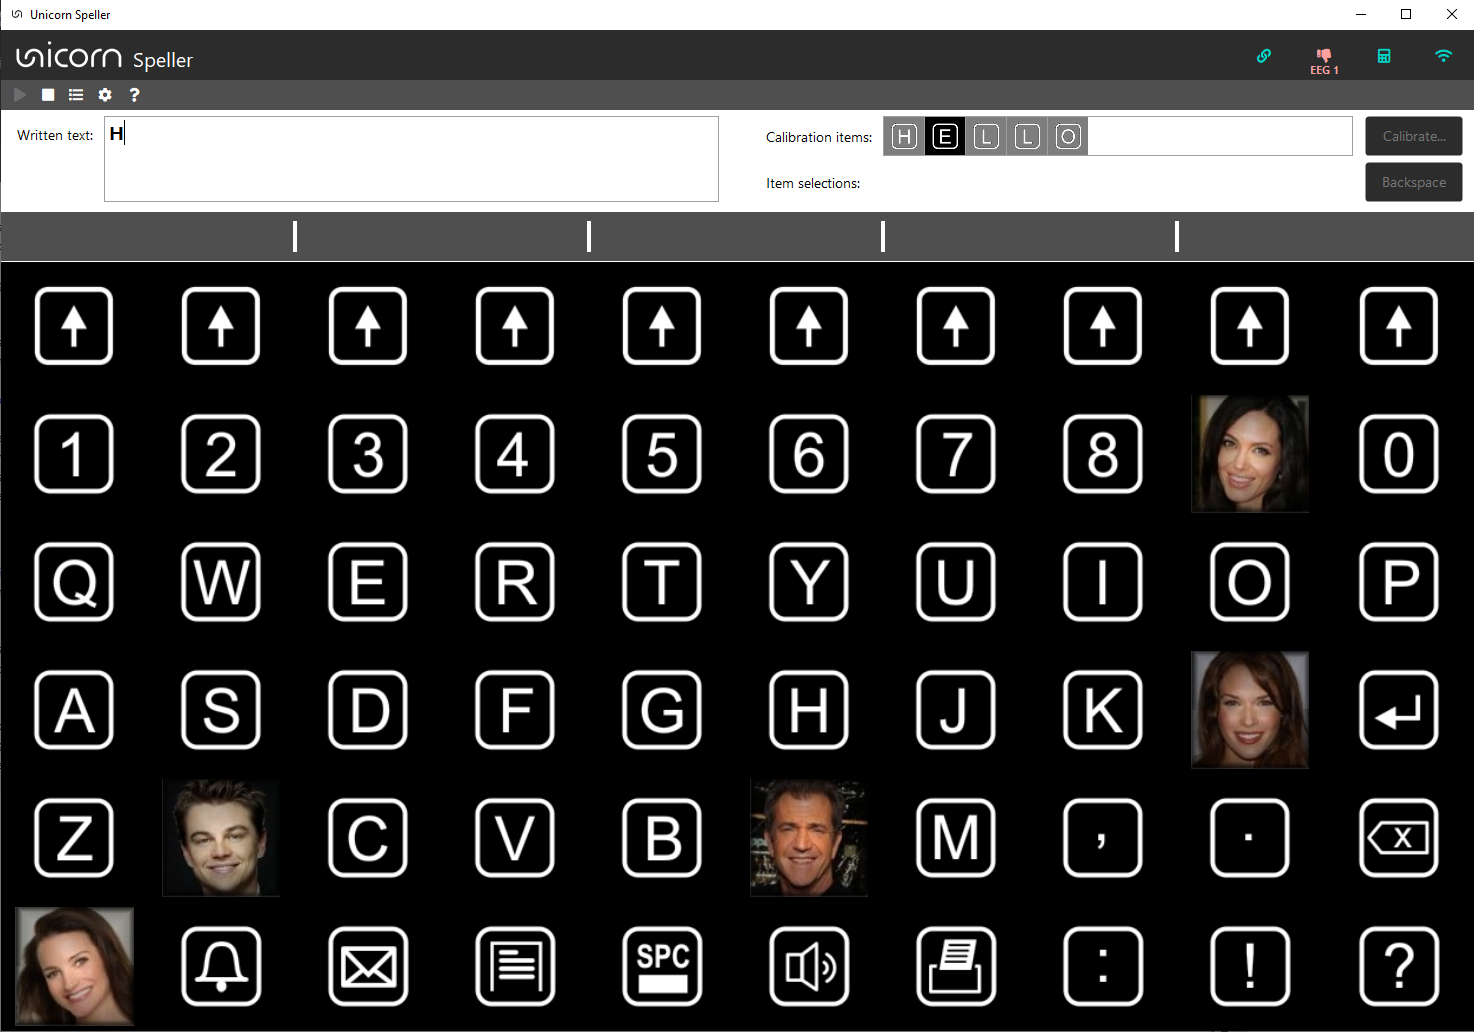
\includegraphics[width=1\textwidth]{Graphics/Speller Calibration.png}
  \caption{Calibration sequence}
\end{figure}
\vspace{\baselineskip}


\subsection{Unity Game Engine}
The Unity engine is a game development platform created by Unity Technologies that offers multiple solutions for creating both 2D and 3D applications and games. Used in multiple fields such as the automotive industry, engineering and architecture\cite{Unity_engine}, the platform is an easy and intuitive way to create different software implementations. Furthermore, the engine supports cross-platform deployment of applications, making it facile to distribute software solutions without hassle. This feature will however not be taken advantage of in the execution of this work, because the unicorn software doesn't work on UNIX-based systems\cite{UnicornSuite_Manual}.
\vspace{\baselineskip}


\subsection{Visual Studio 2022 IDE}
Visual Studio 2022 is an Integrated Development Environment (IDE) used for editing, debugging, building code and publishing different applications. Visual Studio includes compilers, code completion tools, graphical designers and other features to enhance software development processes\cite{VisualStudio}. Visual Studio also provides plugins and different integration with external tools, such as the Unity Game Engine. In the making of this bachelor's work, the main Development Environment used is the 2022 version of this IDE, both as the default script editor for Unity and in other miscellaneous tasks as a code editor.
\vspace{\baselineskip}\newline
Due to the comprehensive support for Microsoft Foundation Class (MFC) applications, the IDE was also used to create the platform's installer, which is an MFC-type application. Visual Studio has extensive tools for designing the MFC user interface and the logic behind it and was crucial in developing, building, running and deploying the platform's installer.
\vspace{\baselineskip}\newline
For trivial and smaller code editing tasks, the simpler Visual Studio Code was used as a quicker alternative to the vastness of its bigger and more complex counterpart.
\vspace{\baselineskip}\newline


\subsection{Programming Languages Used}
\subsubsection{C\#}
C\# is a modern, innovative, open source and multi-platform Object-Oriented Programming (OOP) language\cite{C_sharp} developed by Microsoft. C\# is one of the top 5 languages used by projects on GitHub and one of the most loved languages on Stack Overflow\cite{StackOverflow_language_survey}. The language is a high-level programming language, featuring garbage collection for better memory management. It is also the primary language used for scripting in the Unity game engine. Inside the engine, the language is used to create scripts that control app behaviour by attaching said scripts to in-engine objects to control their behaviour. They can also be used to control global application properties inside Unity. As such, it is the main language used in creating the graphical user interface of the platform and it is also used for creating the speller receiver, a script that asynchronously awaits input from the Unicorn BCI.

\subsubsection{Visual C++}
Visual C++ is a programming language and development environment provided by Microsoft which is a version of the C++ language with added support for Windows-based development. Visual C++ is part of the Visual Studio IDE, making the development process much easier through the use of the powerful IDE's tools. The language also has .NET support, making the use of .NET libraries possible. Its compiler is also highly capable, being able to generate highly optimised machine code for the Windows platform.

\subsubsection{Batch Scripting}
While not a programming language, batch scripting consists of a series of commands that are then executed on a line-by-line basis by the shell program (in this case cmd.exe). Batch files are used to simplify routine and repetitive tasks. A file of this type is an unformatted text file that consists of one or more commands bearing the file extension \textit{.bat} or \textit{.cmd}. After a run, the batch file returns a value of 0 if the run went smoothly or a value of 1 if errors occurred during the execution of the batch file\cite{batch_files}. In this project, batch files are used inside the installer tool application to execute system calls, move apps across the file system and send requests to GitHub.
\vspace{\baselineskip}\newline


\subsection{GitHub}
GitHub is a hosting platform for version control and collaboration\cite{github_HelloWorlds}. It was founded on Git, an open-source code management system created by Linus Torvalds. Git is widely used in the programming community for storing code and tracking the history of said code from its inception. Another key feature is collaboration, with Git allowing developers to collaborate on a project, providing code conflict resolution tools. GitHub provides a web interface for the Git code repository alongside other collaboration and management tools\cite{whatsGithub}. During the development of this thesis, GitHub was used as a versioning system for the platform application, the installer application and the LaTeX thesis, the present document, itself.
\vspace{\baselineskip}\newline
Alongside the present bachelor's work, all the BCI applications developed by me and my colleagues during our Bachelor's degree at the West University of Timisoara are also stored and versioned on the website. The release feature on the website is used to store binary files containing executables for easy downloading, with each application having its own release. Using the GitHub API to send requests to the platform, the aforementioned binaries can be downloaded from the command line. This is the mechanism that stands behind the installer tool, making it possible to grab all applications at once and store them on the user's computer.

